\documentclass[sigconf,nonacm]{acmart}
\pagestyle{plain}
\usepackage{graphicx}
\usepackage{booktabs}
\usepackage{tabularx}
\usepackage{placeins}
\usepackage{needspace}

\raggedbottom
\widowpenalty=10000
\clubpenalty=10000
\displaywidowpenalty=10000

\begin{document}

\title{Working Title Placeholder}
\subtitle{Full Research Paper}

\author{Author Name}
\affiliation{
  \institution{Institution Name}
  \city{City}
  \country{Country}
}
\email{author@example.com}

\begin{abstract}
This paper presents the current DNAT marketplace architecture as a security-oriented design for confidential data processing in data marketplaces. The system combines a blockchain-based access-control layer, IPFS-based artifact distribution, an isolated build service, and an isolated execution service based on Firecracker microVMs. The central design claim is that confidential marketplaces should not only isolate runtime execution, but should also separate control, dependency resolution, and data processing into distinct trust domains with different persistence and network properties.

The paper therefore evaluates the architecture primarily as a compartmentalization strategy. Instead of asking whether the platform is perfectly trusted, the relevant question is whether compromise in one phase can propagate toward all other assets. The DNAT design answers this by ensuring that the build plane persists only wheel artifacts, the execution plane runs without network access, and the control plane does not directly install third-party Python dependencies. This decomposition is contrasted with a centralized baseline in which control logic, execution, sensitive storage, and external connectivity remain colocated.

The main argument of the paper is comparative: the current design is justified because it reduces blast radius, narrows lateral-movement opportunities, and limits post-compromise persistence better than simpler alternatives. At the same time, the paper explicitly discusses the cost of this choice, including added operational complexity, latency overhead, residual trust in the control plane, incomplete service-to-service authentication, and the need for a stronger confidentiality treatment for dataset handling. The goal is not to overclaim trustlessness, but to defend the architecture as a credible high-assurance baseline for a confidential marketplace prototype.
\end{abstract}

\keywords{Confidential computing, data marketplace, Firecracker, isolation, security architecture}

\maketitle

\Needspace{12\baselineskip}
\section{Introduction}

Confidential data marketplaces must simultaneously support asset exchange, access control, and third-party computation over sensitive inputs. That combination creates a difficult systems problem. A marketplace that accepts externally supplied applications cannot treat code execution as an isolated implementation detail, because the same platform also handles persistent metadata, payment and access logic, storage backends, and the datasets that motivate the marketplace in the first place. In practice, the problem is not merely how to ``run code safely,'' but how to prevent build-time and run-time compromise from expanding into a full platform compromise.

The most direct implementation path would be a centralized confidential virtual machine that hosts the marketplace-facing logic, local artifact storage, and the execution orchestrator in the same trust domain. That design is operationally attractive because it minimizes deployment complexity and avoids inter-service coordination. However, it also creates the wrong security shape for the problem: the same node that validates access and manages persistent sensitive state also becomes the place where untrusted or semi-trusted workloads are prepared and executed.

\begin{figure*}[t]
\centering
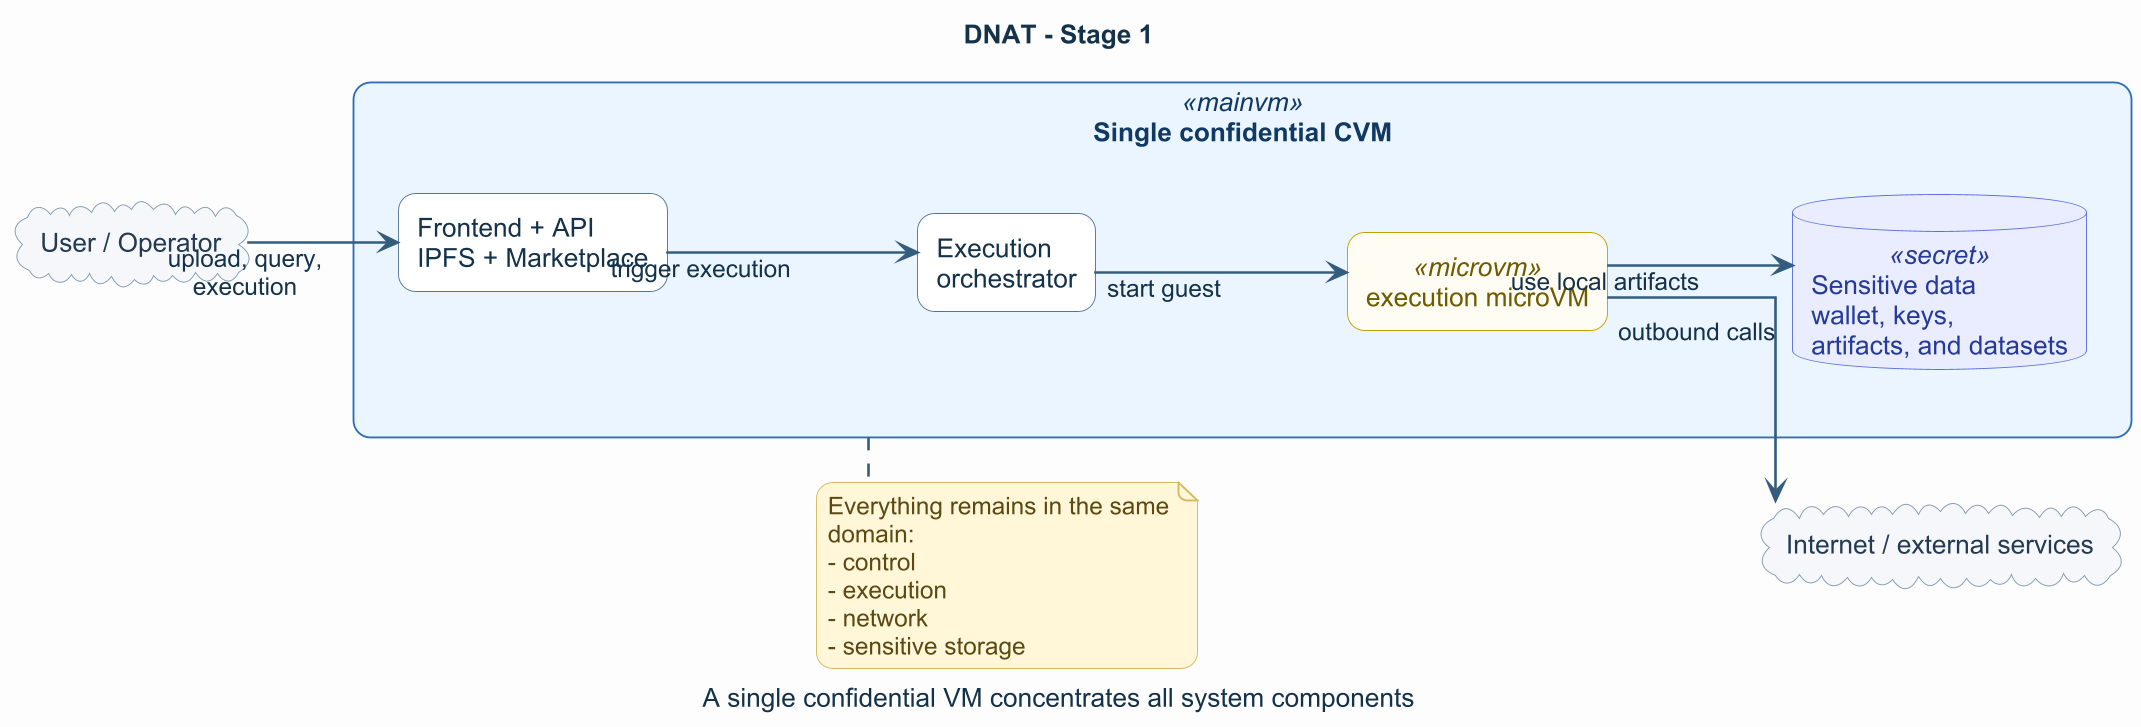
\includegraphics[width=0.86\textwidth]{figures/architecture-evolution-01-single-cvm.png}
\caption{Centralized baseline architecture. Its operational simplicity is attractive, but the control plane, local sensitive storage, and execution path remain in the same trust domain.}
\Description{A two-column-wide diagram showing a single confidential virtual machine containing the frontend, marketplace, execution orchestrator, execution microVM, and sensitive data store. It highlights that control, execution, network access, and sensitive storage are colocated in the same trust domain.}
\label{fig:single-cvm}
\end{figure*}

Figure~\ref{fig:single-cvm} captures the baseline that this paper argues against. In such a layout, compromise in the execution path can more easily pivot toward locally stored artifacts, wallet-related material, marketplace state, or any other control-plane asset colocated in the same environment. The architecture implemented in this repository was developed precisely to avoid that concentration of privilege.

The thesis of this paper is that the current three-layer design is justified because it reduces privilege concentration and constrains failure propagation better than simpler alternatives. The central claim is not that each component is individually invulnerable, but that compromise in one stage does not automatically grant access to all other assets. This matters in data marketplaces because the platform must simultaneously handle datasets, application artifacts, dependency resolution, access checks, execution results, and persistent metadata.

The contributions of this paper are as follows:
\begin{itemize}
\item an implementation-oriented description of the DNAT architecture, emphasizing trust boundaries and persistence rules;
\item a security argument for keeping build isolation and execution isolation as separate concerns;
\item a discussion of residual weaknesses and of alternative architectures that introduce additional attack paths.
\end{itemize}

Taken together, these contributions position the work as a security architecture paper rather than only as a deployment report. The objective is to explain why the current implementation is structured as it is, what security properties that structure is intended to support, and where the remaining trust assumptions still lie.

The remainder of this paper is organized as follows. Section~2 discusses background and situates the work. Section~3 defines the scope and threat model. Section~4 presents the DNAT architecture and the rationale behind its decomposition. Section~5 analyzes the resulting security properties and trade-offs. Section~6 summarizes the main threats and mitigations. Section~7 describes an evaluation methodology aligned with the design claims. Section~8 discusses the broader significance and limitations of the approach, and Section~9 concludes the paper.

\section{Related Work and Background}

The problem addressed by this paper intersects at least three areas of prior work: confidential execution environments, secure data-processing platforms, and systems architectures for isolating untrusted computation. The first area contributes the general intuition that sensitive computation should be executed in a constrained environment with reduced visibility into the rest of the system. The second area contributes the observation that data-processing platforms often combine persistent metadata, user-facing orchestration, and external code or plugins in ways that create broad attack surfaces. The third area contributes the architectural principle that isolation boundaries are not merely runtime controls, but system-design choices that shape failure propagation.

In the context of this paper, the most relevant background distinction is between \emph{execution isolation} and \emph{system isolation}. Execution isolation alone focuses on constraining the code that processes the dataset. System isolation, by contrast, asks a broader question: where are dependencies resolved, where are artifacts stored, which component can reach network resources, and which component retains sensitive persistent state. This distinction is central because a marketplace architecture can include a strongly isolated execution environment while still leaving the control plane or build path excessively exposed.

Another useful distinction is between a \emph{centralized trust domain} and a \emph{compartmentalized trust domain}. In the former, orchestration logic, storage, external communication, and untrusted workload preparation remain colocated, which simplifies deployment but increases coupling between failures. In the latter, those concerns are separated across components with different reachability and persistence rules. This paper adopts the second approach and argues that such compartmentalization is better suited for confidential data marketplaces.

\section{Scope and Threat Model}

The threat model is driven by the fact that the system accepts externally supplied applications and resolves their dependencies before allowing them to process protected datasets. The most relevant assets are therefore: (i) datasets and application artifacts, (ii) marketplace metadata and access-control state, (iii) wallet or signing material bound to marketplace actions, (iv) reusable build artifacts such as cached wheels, and (v) execution outputs and logs.

The main adversarial scenarios considered in this work are the following. First, a malicious application author may try to use the submitted code or dependency graph to escape the execution environment, exfiltrate datasets, or persist malicious state across runs. Second, a malicious or compromised dependency may attempt supply-chain abuse during the build phase, where package installation and artifact generation are allowed to execute complex external code. Third, an attacker who compromises a less privileged component may try to move laterally toward marketplace metadata, stored assets, wallet material, or future executions. Fourth, a passive or active network adversary may benefit from weak service identity if internal communication is not strongly authenticated.

The design partially addresses these scenarios by constraining component reachability and by minimizing what each layer can store or access. However, the implementation does \emph{not} currently remove all trust from the infrastructure. The control plane remains privileged, internal communication does not yet implement mutual TLS, and the repository does not expose a complete remote attestation flow that would let an external party verify the precise software state of all confidential components before use. Therefore, the paper should avoid absolute claims about end-to-end trustlessness or about fully decentralized trust.

Another important assumption concerns dataset handling. The current code clearly encrypts the built application artifact before it is published to IPFS, but dataset confidentiality depends on how the dataset is prepared before registration and on how the control plane handles it during execution orchestration. This should be stated as an implementation limitation or as a deployment assumption, not hidden behind generic confidentiality claims. The system is therefore better described as \emph{execution-isolating by design} than as already providing a fully verified end-to-end confidentiality pipeline for every stored asset.

The threat model also has clear boundaries. The paper does not claim to solve malicious host administrators, physical attacks against the underlying infrastructure, or side-channel attacks on confidential-computing substrates. These issues are important, but they are not the primary design axis of the current implementation. The architecture is instead optimized around containing application-level, dependency-level, and service-boundary compromise within a practical marketplace prototype.

\section{DNAT Architecture}

\Needspace{12\baselineskip}
The current implementation is organized around three components. \textbf{CVM1} hosts the client-facing logic, including the local marketplace interface, the blockchain interaction layer, IPFS integration \cite{benet2014ipfs}, and artifact encryption before application publication. \textbf{CVM2} is a dedicated build service that receives application bundles from CVM1 and spawns an ephemeral Firecracker microVM to resolve dependencies and produce an \texttt{application.ext4} artifact. \textbf{CVM3} is a dedicated execution service that receives a temporary execution bundle and launches an ephemeral Firecracker microVM without network access. The build and execution environments rely on Firecracker-style microVM isolation \cite{agache2020firecracker}.

This separation is important because each component persists different classes of data. CVM1 retains marketplace state and published blobs, CVM2 persists only reusable wheel files, and CVM3 is reduced to runtime artifacts needed to launch isolated executions. Temporary data are removed after build and execution, limiting cross-request contamination. The repository documentation already reflects this design through architecture diagrams, build scripts, and runtime cleanup procedures.

\begin{figure*}[t]
\centering
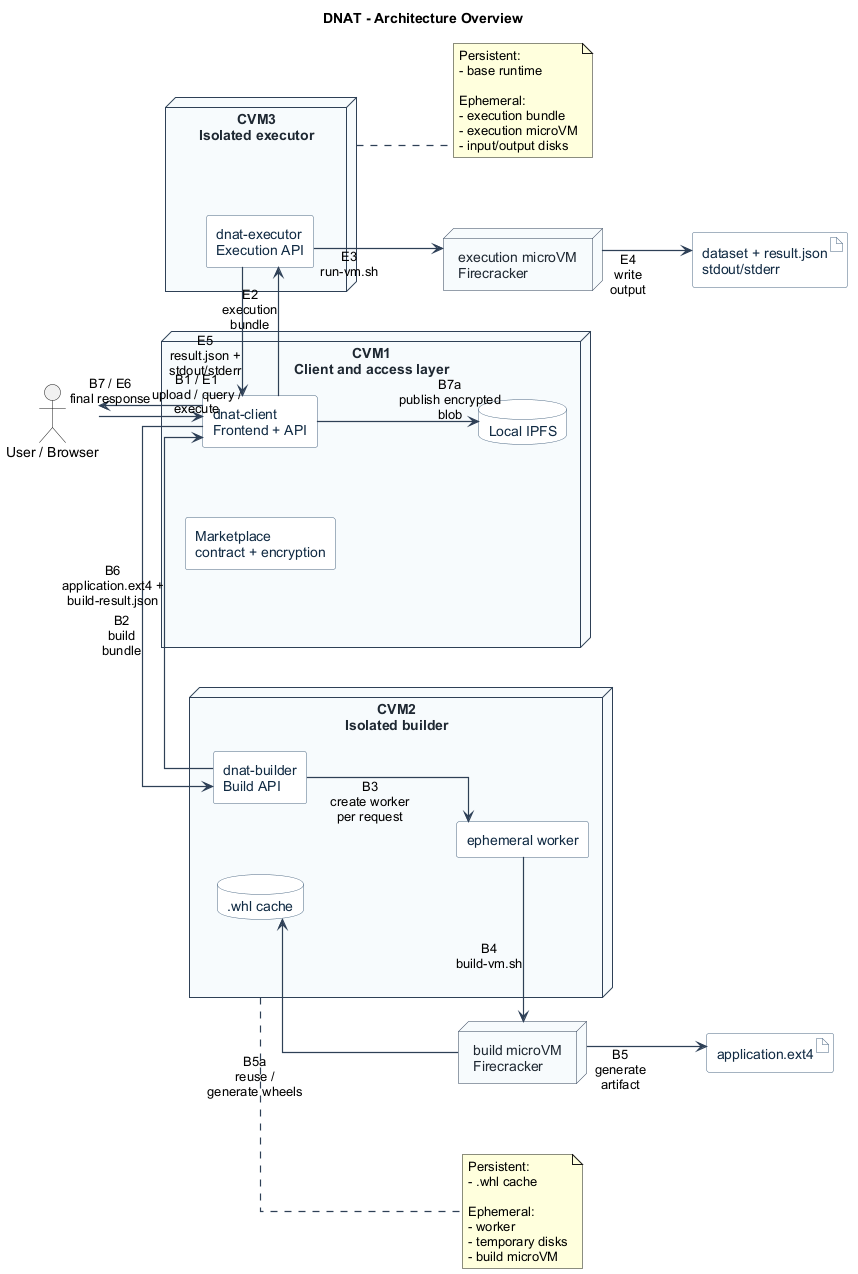
\includegraphics[width=0.78\textwidth]{figures/architecture-overview.png}
\caption{High-level view of the current DNAT architecture. The main value of this figure is clarity: it shows the separation between the control plane, the isolated build plane, and the isolated execution plane.}
\Description{A two-column-wide architecture overview showing three components: CVM1 as the client and access layer with frontend, API, marketplace, and local IPFS; CVM2 as the isolated builder with build API, ephemeral worker, and wheel cache; and CVM3 as the isolated executor with execution API and execution microVM. The arrows depict build and execution bundles and the publication of an encrypted blob to IPFS.}
\label{fig:architecture-overview}
\end{figure*}

Figure~\ref{fig:architecture-overview} provides the positive counterpart to Fig.~\ref{fig:single-cvm}. Instead of one broad trust domain, the system is decomposed into a control plane, a build plane, and an execution plane. This decomposition is the main architectural move of the paper. It does not magically remove trust, but it changes where trust is required and what a compromised component can still reach.

Figure~\ref{fig:registration-sequence} is particularly relevant because many of the system's most dangerous operations happen before a buyer ever executes an application. Dependency resolution, package download, native wheel compilation, and artifact construction all happen in the build path. If the paper is to justify a dedicated builder, this figure is where the argument becomes concrete.

From a workflow perspective, application registration and application execution are intentionally decoupled. Registration sends the source bundle to the build plane, stores the built application artifact, and publishes only the resulting encrypted blob. Execution later retrieves the dataset and application artifact through the control plane, prepares a temporary workspace, and forwards only the execution bundle to the isolated runtime. This distinction is essential to the security argument because build-time code and run-time data are not treated as the same trust problem. A marketplace that collapses those two phases into one execution environment gains simplicity at the cost of broader compromise semantics.

\begin{figure*}[t]
\centering
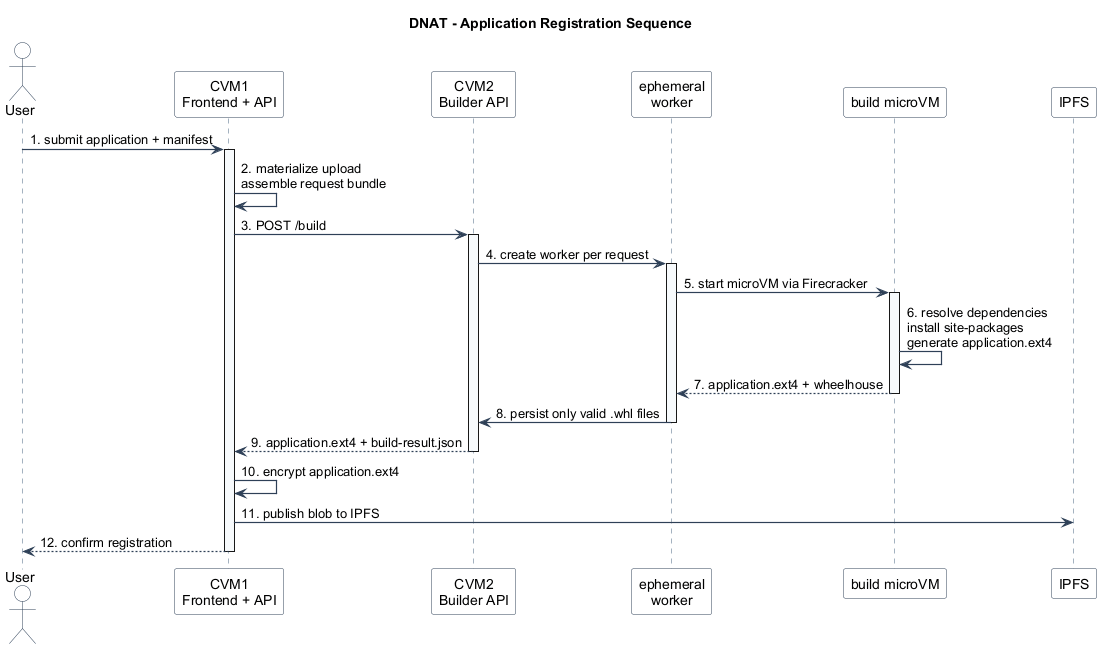
\includegraphics[width=0.72\textwidth]{figures/application-registration-sequence.png}
\caption{Application registration flow. This figure is useful because it makes the build isolation argument concrete: dependency resolution occurs in the builder path before the encrypted artifact is published.}
\Description{A sequence diagram of application registration. The user submits an application and manifest to CVM1, which assembles a build bundle and sends it to the builder API in CVM2. CVM2 creates an ephemeral worker, launches a build microVM, resolves dependencies, generates application.ext4, persists only valid wheel files, returns the artifact to CVM1, and CVM1 encrypts and publishes the result to IPFS.}
\label{fig:registration-sequence}
\end{figure*}

\subsection{Design Goals}

The architecture is designed around four goals. First, the control plane should avoid directly executing dependency installation logic for user-supplied applications. Second, the execution path should minimize straightforward exfiltration channels. Third, artifacts and temporary state should be kept as ephemeral as possible outside the minimum persistence required for system operation. Fourth, the architecture should make post-compromise reasoning simpler by ensuring that different phases of the workflow occupy different failure domains.

\subsection{Centralized Baseline Versus Compartmentalized Design}

The centralized baseline shown earlier represents the simplest implementation strategy: keep storage, orchestration, execution, and external communication together. The DNAT architecture rejects this strategy in favor of a split design where the control plane, builder, and executor are isolated from one another. The motivation is not simply defense in depth as a general slogan, but a more specific reduction in security coupling between unrelated responsibilities.

\subsection{Why the Control Plane Should Not Build Applications}

Keeping dependency resolution outside CVM1 is one of the strongest design decisions in the current implementation. The control plane is the most security-sensitive part of the system because it touches marketplace state, IPFS operations, access validation, and the orchestration of publication and execution. If dependency installation happened in the same component, any malicious package, build hook, or native extension would execute in the same administrative context as the marketplace layer. That would turn a supply-chain problem into a platform compromise.

The current design breaks that path. CVM2 exposes only a minimal build API, persists only wheel files, and uses an ephemeral worker plus an ephemeral build microVM. Even when outbound network access is needed to download packages, the build script explicitly blocks access to private address ranges on the host side. This does not eliminate supply-chain risk, but it narrows the assets that a successful build compromise can reach. In other words, the build plane remains a high-risk locus, but it becomes a \emph{contained} high-risk locus rather than a bridge into the entire platform.

\subsection{Why the Execution Plane Should Stay Separate from the Build Plane}

Combining build and execution into the same isolated host would look simpler, but it would also couple two threat classes that should remain distinct. Build logic needs egress to download dependencies, whereas the execution path should be as closed as possible because it handles the dataset-processing step. If the same environment is reused for both phases, the runtime inherits more tools, more state, and more opportunities for persistence than necessary. It also becomes harder to reason about which artifacts are trustworthy outputs of a past build and which artifacts are leftovers from a prior execution.

The current implementation avoids that coupling. The execution microVM does not receive a network interface, mounts the application artifact read-only, uses a temporary input bundle, and returns results through a persistent output disk collected by the host after shutdown. This sharply limits outbound exfiltration opportunities and keeps the runtime contract narrow: execute the packaged workload, write the result, and terminate. That narrow contract is architecturally valuable because it makes the executor easier to harden and easier to reason about than a multi-purpose host that both builds and runs arbitrary code.

\subsection{Why Ephemeral State Matters}

The architecture depends heavily on the distinction between persistent and ephemeral data. The build plane keeps wheel files but discards the application state after each request. The execution plane removes temporary overlays, disks, mounts, and the Firecracker socket after each run. These cleanup rules are not cosmetic details; they are central to the argument that compromise impact should be bounded in time and scope. In a marketplace setting, persistence is not only a storage concern; it is also a security concern because any leftover writable state can become a covert channel, a persistence foothold, or a contamination vector for later users.

This ephemeral strategy also creates a cleaner narrative for the paper. Instead of claiming that confidential execution magically solves all security issues, the system can be presented as a layered containment strategy: reduce what is reachable during each phase, reduce what survives each phase, and reduce what each compromised component can reveal about the rest of the platform.

\begin{figure*}[t]
\centering
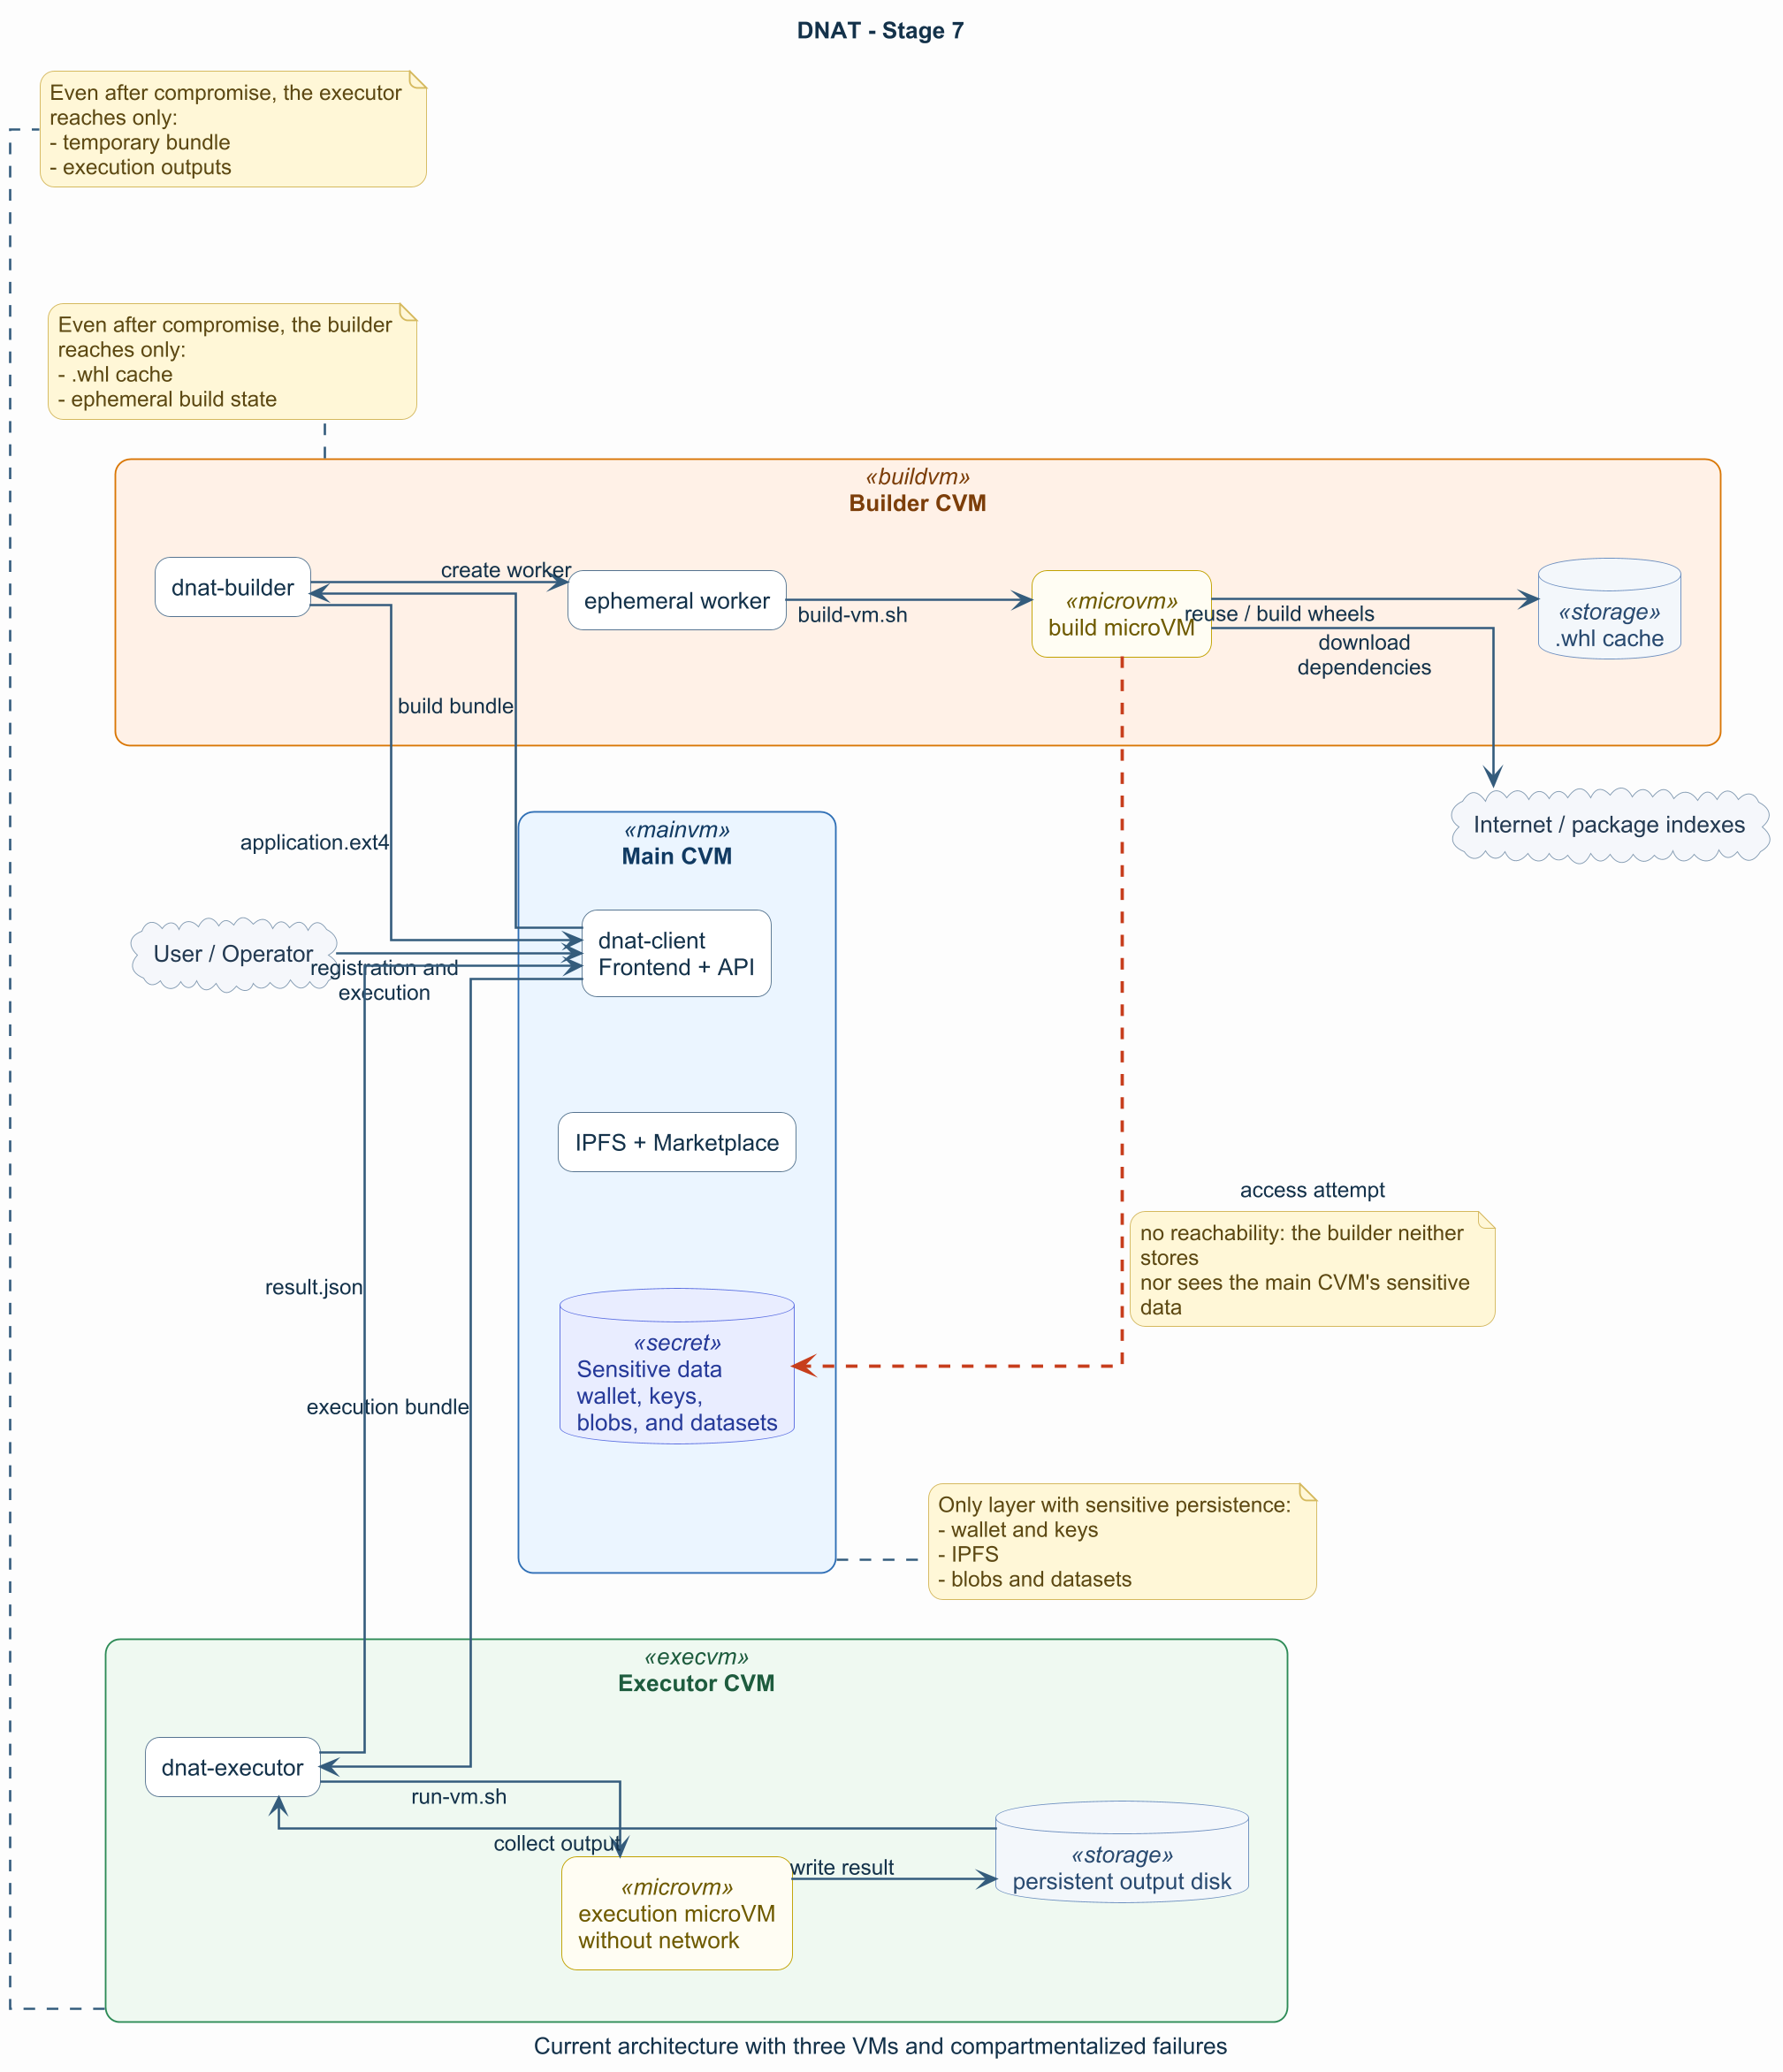
\includegraphics[width=0.92\textwidth]{figures/architecture-evolution-07-three-vm-final-architecture.png}
\caption{Final compartmentalized architecture. This figure supports the core claim of the paper: compromise in the build or execution plane does not immediately expose the full set of sensitive assets held by the control plane.}
\Description{A two-column-wide architecture diagram showing three separate virtual machines: a main control CVM containing the frontend, IPFS, marketplace, and sensitive persistent data; a builder CVM with a build API, ephemeral worker, build microVM, and wheel cache; and an executor CVM with an execution API, networkless execution microVM, and persistent output disk. Dashed annotations indicate that a compromise in the builder or executor cannot directly reach the sensitive data of the main CVM.}
\label{fig:final-architecture}
\end{figure*}

Figure~\ref{fig:final-architecture} should be read as a failure-containment diagram rather than merely as an implementation diagram. Its value is that it makes visible what the paper is really defending: the build plane can fail without inheriting control-plane secrets, and the execution plane can fail without automatically acquiring the network and storage privileges of the builder or the marketplace layer.

\FloatBarrier
\Needspace{12\baselineskip}
\section{Security Analysis}

\Needspace{10\baselineskip}
\subsection{Positive Aspects of the Current Design}

The first major advantage is \textbf{blast-radius reduction}. A compromise in the execution microVM does not automatically expose the local IPFS node, the blockchain client, or the build cache because those resources are outside the execution environment. The second advantage is \textbf{phase-specific hardening}. The build phase tolerates limited outbound connectivity but blocks private destination ranges, while the execution phase removes network access entirely. The third advantage is \textbf{minimal persistence}. The build plane persists only wheel files, and the execution plane is designed to die cleanly after each run.

The fourth advantage is \textbf{artifact immutability during execution}. The execution host mounts \texttt{application.ext4} read-only, which reduces the risk that a single run silently mutates the packaged application for later reuse. The fifth advantage is \textbf{narrow interfaces}. Both the build plane and the execution plane are invoked through small service APIs instead of exposing general-purpose shells or shared storage to the control plane. The sixth advantage is \textbf{cleaner security reasoning}. Because responsibilities are split by phase, the system can justify different hardening choices for each component instead of forcing one broad compromise between convenience and containment.

\Needspace{10\baselineskip}
\subsection{Negative Aspects and Residual Risk}

The current architecture also has non-trivial drawbacks. The first is \textbf{operational complexity}. Three components, temporary disks, Firecracker orchestration, and containerized deployment increase engineering and debugging cost. The second is \textbf{latency overhead}. Build and execution both pay setup and teardown costs that a monolithic design would avoid. The third is \textbf{control-plane trust concentration}. CVM1 still orchestrates the workflow and remains a high-value target.

There are also security gaps that should be discussed honestly. Internal service authentication is still incomplete because the repository documentation explicitly notes that mutual TLS is not implemented. Dataset confidentiality handling is weaker than the application-artifact path and should be tightened before making stronger confidentiality claims. The current design also does not yet expose a strong attestation story that would let an external stakeholder verify the software identity of each confidential component before trusting the result. Finally, wheel caching improves performance, but it remains a supply-chain sensitive mechanism and should be treated as a controlled optimization rather than a free security win.

These limitations are not peripheral details; they are part of what makes the argument publishable. A stronger article is one that distinguishes clearly between the security properties the implementation already enforces and the properties that remain future work. In this case, the most defensible claims concern containment, separation of duties, and reduction of straightforward exfiltration and persistence paths. Claims about complete confidentiality, complete trust minimization, or comprehensive attestation would currently be harder to support.

\Needspace{10\baselineskip}
\subsection{Why Simpler Alternatives Increase the Attack Surface}

A single-VM architecture would collapse trust boundaries and make lateral movement easier. Malicious code could target the same filesystem namespace that contains marketplace data, execution outputs, IPFS state, or private blockchain material. A shared build-and-run environment would also let build-time tools survive long enough to affect later executions. Likewise, enabling network access inside the execution microVM would reintroduce exfiltration channels, command-and-control paths, and metadata probing opportunities that the current executor intentionally avoids.

The problem with the centralized baseline is not merely that it is ``less secure'' in an abstract sense. The problem is that it creates \emph{security coupling}. In a coupled design, the same local compromise may simultaneously threaten confidentiality of stored assets, integrity of marketplace decisions, and availability of future executions. By contrast, the current architecture tries to turn one large failure domain into several smaller ones. That is the central comparative argument of the paper.

The most important argumentative move for the paper is therefore comparative rather than absolute: the current architecture should be defended because it is safer than simpler alternatives under realistic implementation constraints, not because it eliminates every attack class.

\FloatBarrier
\Needspace{12\baselineskip}
\section{Threats and Mitigations}

\begin{table*}[t]
\centering
\caption{Threats and architectural mitigations.}
\label{tab:attacks}
\footnotesize
\begin{tabularx}{\textwidth}{@{}p{3.1cm}p{4.6cm}X@{}}
\toprule
Attack & Why it matters & Current architectural answer \\
\midrule
Dependency-based compromise during build & Malicious packages may execute arbitrary code while dependencies are resolved. & Build happens in CVM2 through an ephemeral worker and an ephemeral build microVM; private host ranges are blocked during package download; only wheel files are retained after the build. \\
\addlinespace
Runtime data exfiltration & Buyer code may try to leak sensitive dataset contents. & The execution microVM is launched without a network interface and returns results only through a collected output disk. \\
\addlinespace
Cross-run persistence & One execution may try to plant tools or modified state for future runs. & Temporary overlays, input disks, output disks, mounts, and Firecracker sockets are removed after execution; the application artifact is mounted read-only. \\
\addlinespace
Lateral movement toward marketplace services & A runtime compromise may attempt to reach IPFS, wallet material, or smart-contract logic. & Execution is separated from the control plane, and the executor does not host marketplace services or IPFS. \\
\addlinespace
Cache poisoning or unsafe artifact reuse & Build optimizations may become a persistence or tampering channel. & CVM2 ingests only \texttt{.whl} files, validates names, rejects oversized files, and prunes the cache by size; however, stronger provenance validation is still desirable. \\
\addlinespace
Internal service impersonation & A forged internal service could feed malicious build or execution results. & This remains a gap in the current repository because mutual TLS and stronger service identity are still pending. \\
\bottomrule
\end{tabularx}
\end{table*}

\FloatBarrier
\Needspace{12\baselineskip}
\section{Evaluation Methodology}

The architecture argument becomes substantially stronger if it is tied to explicit evaluation criteria. In this context, the most relevant criteria are: (i) compromise containment, meaning whether a failure in one phase reaches unrelated assets; (ii) exfiltration resistance, meaning whether execution-time code can open obvious outbound channels; (iii) persistence resistance, meaning whether one run can contaminate later runs; and (iv) operational cost, meaning the latency and complexity introduced by the isolation strategy.

The paper can therefore evolve from a purely architectural description into a practical security study by validating a small set of claims experimentally. First, the build path can be tested with a deliberately hostile dependency or build script to show that compromise is contained inside the build plane and does not grant direct access to marketplace assets. Second, the runtime can be tested with an application that attempts outbound network communication, proving that the current executor blocks that behavior by construction. Third, persistence claims can be validated by checking that temporary execution artifacts disappear after each run. Fourth, the centralized baseline can be used as a comparative mental model to explain why each blocked action would have been more dangerous in a less compartmentalized design.

It is also useful to evaluate the tradeoff side of the design. The paper should measure build latency, execution latency, and artifact size overhead introduced by the isolation layers. Those numbers will help justify the claim that the architecture buys meaningful risk reduction at an acceptable engineering cost for a confidential marketplace setting. Without such measurements, the argument remains conceptually strong but empirically incomplete.

The experimental section can be strengthened with security testing tools that target different layers of the system. Static analyzers such as Semgrep and Bandit can inspect the orchestration code for unsafe patterns. Supply-chain tools such as pip-audit, Syft, and Grype can expose dependency and artifact risk in the build path. Container and image scanners such as Trivy are relevant for the CVM images themselves. Dynamic tools such as Nmap, curl, and custom proof-of-concept workloads can validate that the executor remains unreachable from the outside and that the guest cannot perform the outbound actions that a less isolated architecture would allow. Network observation tools such as tcpdump or Wireshark can provide concrete evidence that the executor lacks the exfiltration channel that the centralized baseline would have left available.

For the paper to read as a high-quality systems-security article, the evaluation should not merely list successful checks. It should connect each test to a design claim. For example, a failed outbound connection from the executor is evidence for exfiltration resistance; absence of leftover overlays is evidence for persistence resistance; and unsuccessful access from the builder toward private address ranges is evidence that the build plane is constrained even when it needs egress for package retrieval.

\Needspace{12\baselineskip}
\section{Discussion}

The structure adopted in this paper intentionally mirrors a pattern common in strong LADC papers: a clear problem statement, explicit scoping assumptions, a technical core section that defines the proposal, and a separate analytical section that explains why the proposal matters. For this work, the most important discussion point is that the architecture should be judged neither as a generic marketplace implementation nor as a fully solved confidential-computing platform. Its proper evaluation target is narrower and more defensible: whether the implemented decomposition meaningfully improves containment over plausible simpler baselines.

From that perspective, the architecture has a strong argument. It treats build, control, and execution as different trust problems. It reduces obvious runtime exfiltration paths. It narrows persistent state in the builder and executor. It also leaves clear room for future work, particularly in stronger service identity, attestation, and dataset confidentiality handling. This combination of concrete present-day containment and explicit future-work boundaries is more appropriate for a high-quality dependability and security paper than an overly broad claim of complete protection.

\Needspace{12\baselineskip}
\section{Conclusion}

This draft frames the DNAT implementation as a layered containment architecture rather than a generic marketplace prototype. Its main value is the explicit separation of control, build, and execution concerns, combined with ephemeral microVM-based processing and constrained persistence. That separation provides a defensible answer to attacks involving untrusted application code, dependency resolution, and lateral movement across platform responsibilities.

At the same time, the architecture should be presented with precise limits. The control plane is still privileged, internal mutual authentication is incomplete, and dataset confidentiality deserves stronger treatment in the implementation. These limitations do not weaken the paper if they are discussed directly; instead, they make the argument more credible by showing that the design is security-conscious without overstating what has already been achieved.

\bibliographystyle{ACM-Reference-Format}
\bibliography{references}

\end{document}
